\documentclass[11pt]{article}
\usepackage[a4paper,margin=1in]{geometry}
\usepackage[T1]{fontenc}
\usepackage[utf8]{inputenc}
\usepackage{lmodern}
\usepackage{microtype}
\usepackage{amsmath,amssymb}
\usepackage{booktabs}
\usepackage{array}
\usepackage{tabularx}
\usepackage{enumitem}
\usepackage{listings}
\usepackage{xcolor}
\usepackage{tikz}
\usetikzlibrary{positioning,arrows.meta,shapes.geometric,fit,backgrounds,calc}
\usepackage{url}
\usepackage{xltabular}
\usepackage[hidelinks]{hyperref}

\definecolor{accent}{HTML}{1F5FA8}
\definecolor{good}{HTML}{2E7D32}
\definecolor{bad}{HTML}{C62828}
\definecolor{warn}{HTML}{E09A1A}
\definecolor{quiet}{HTML}{6B6B6B}
\definecolor{tintbg}{HTML}{F3F2EE}

\lstset{basicstyle=\ttfamily\small,columns=fullflexible,keepspaces=true,
  breaklines=true,frame=single,framerule=0.3pt,rulecolor=\color{quiet},
  xleftmargin=1em,xrightmargin=1em,aboveskip=0.8em,belowskip=0.8em}

\newcolumntype{L}[1]{>{\raggedright\arraybackslash}p{#1}}
\setlist{nosep}
\emergencystretch=3em \tolerance=3000 \hfuzz=0.5pt
\renewcommand{\arraystretch}{1.15}

\newcommand{\code}[1]{\texttt{#1}}
\newcommand{\subtxt}{\footnotesize\color{quiet}}
\newcommand{\dev}{\code{dev}}
\newcommand{\ote}{\path{feature/rev-stacks-ote}}

\title{Node-Local Deploy Queues and the \code{f1r3node-async-rust} Client\\
  {\large A design note for \code{f1r3node-rust}}}
\author{L.\,G.\ Meredith\\ F1R3FLY.io}
\date{7 November 2026 \quad (surveyed at \dev{} \code{a79a6ce}, \ote{} \code{4c9853b})}

\begin{document}
\maketitle

\begin{abstract}
A shard should absorb a burst of deployments from many clients without stalling.
This note designs two components that make that so: a pairing of each
\code{f1r3node} with its own RabbitMQ queue, drained by a consumer task inside the
node that hands each message to the existing deploy path; and an async Rust client
that signs a deploy, publishes it to a node's queue, and follows its fate through
status events. The queue is strictly node-local, so no shared service can take the
network down. The deploy's block-window validity stays as the mechanism that bounds a
backlog; it is already a shard-wide genesis parameter on both branches surveyed, so
no new consensus parameter is needed. Everything branch-specific sits behind one
seam, \code{BlockAPI::deploy}, which the design does not cross, so one
implementation serves current \dev{} and the cost-accounting branch intended for the
ASI TestNet.
\end{abstract}

\tableofcontents

\section{Aim and scope}

Two components deliver burst tolerance:
\begin{enumerate}[leftmargin=2em]
  \item \textbf{Node + queue pairing.} Every \code{f1r3node} in the shard runs beside
    its own RabbitMQ broker. A consumer task inside the node receives messages from
    that queue as they arrive---RabbitMQ pushes deliveries to a registered consumer,
    the node never polls---and hands each one to the node's existing deploy path,
    exactly as if it had come from the \code{f1r3node-rust} client over gRPC.
  \item \textbf{\code{f1r3node-async-rust} client.} An async Rust library (and thin
    CLI) that human and agentic clients use to deploy to the shard. It signs the
    deploy, publishes it to a node's queue, and gives the caller an async handle for
    following the deploy's fate.
\end{enumerate}

Three constraints shape the design.
\begin{itemize}[leftmargin=2em]
  \item \emph{No shared broker.} The queue is node-local. There is no central queue
    service whose failure takes down the network; a broker outage affects one node's
    intake only.
  \item \emph{The deploy TTL stays, as a shard-wide parameter.} Deployments already
    expire after a block window. That window remains the mechanism that stops a
    backlog from becoming stale work; its length is set at shard launch, not compiled
    in.
  \item \emph{Works on \dev{} and on the cost-accounting branch.} The design must sit
    on current \dev{} (run-to-completion with merge logic) and on \ote{}
    (cost-accounted order-then-execute). It therefore lives at the deploy-ingress
    seam, above everything the two branches disagree about: execution, charging and
    finality.
\end{itemize}

Out of scope: changing deploy semantics, the consensus protocol, or how the proposer
selects deploys. The queue changes \emph{when} and \emph{how fast} deploys reach the
node, not what the node does with them.

\section{Where this sits in the architecture}

Figure~\ref{fig:arch} is the ``F1R3FLY.io Deployment Architecture'' diagram made
concrete. The DeployQueue beside each F1R3Node is a RabbitMQ broker that only that
node consumes from; the RustAsync-Client box is the \code{f1r3node-async-rust}
library in the client's process. Everything to the right of the queue---consensus,
RSpace, oracle-mode data sources such as SWI-Prolog and FileIO---is unchanged, so the
diagram's invariant holds: all client traffic still enters through a node,
consensus-mode data keeps one view, and oracle-mode data stays tied to the node that
touched it.

\begin{figure}[htbp]
\centering
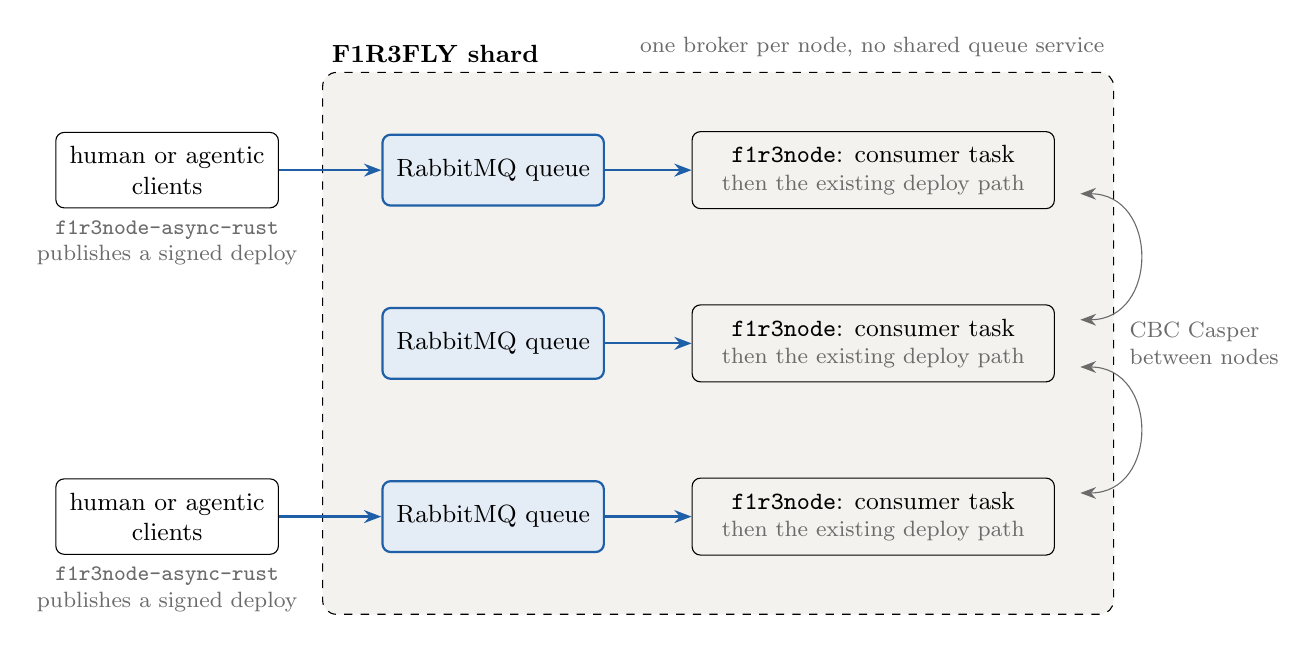
\begin{tikzpicture}[
  font=\small,
  node/.style={draw,rounded corners=3pt,minimum height=0.9cm,align=center,inner sep=5pt},
  queue/.style={node,fill=accent!12,draw=accent,thick},
  client/.style={node,minimum width=2.4cm},
  flow/.style={-{Stealth[length=2.2mm]},accent,thick},
  cons/.style={{Stealth[length=2mm]}-{Stealth[length=2mm]},quiet},
]
\foreach \i/\y in {1/0,2/-2.2,3/-4.4}{
  \node[queue] (q\i) at (0,\y) {RabbitMQ queue};
  \node[node,right=1.1cm of q\i,minimum width=4.6cm] (n\i) {\code{f1r3node}: consumer task\\[-1pt]{\color{quiet}\footnotesize then the existing deploy path}};
  \begin{scope}[on background layer]
    \node[draw,rounded corners=4pt,fit=(q\i)(n\i),inner sep=9pt,label={[anchor=south west,font=\small\bfseries]north west:Validator \i}] (v\i) {};
  \end{scope}
  \draw[flow] (q\i) -- (n\i);
}
\node[client,left=1.3cm of q1] (c1) {human or agentic\\clients};
\node[client,left=1.3cm of q3] (c3) {human or agentic\\clients};
\draw[flow] (c1) -- (q1);
\draw[flow] (c3) -- (q3);
\node[below=1pt of c1,font=\footnotesize,color=quiet,align=center] {\code{f1r3node-async-rust}\\publishes a signed deploy};
\node[below=1pt of c3,font=\footnotesize,color=quiet,align=center] {\code{f1r3node-async-rust}\\publishes a signed deploy};
\draw[cons] (v1.east) ++(0,-0.3) to[out=0,in=0,looseness=1.6] ($(v2.east)+(0,0.3)$);
\draw[cons] (v2.east) ++(0,-0.3) to[out=0,in=0,looseness=1.6] ($(v3.east)+(0,0.3)$);
\node[right=0.5cm of v2.east,font=\footnotesize,color=quiet,align=left] {CBC Casper\\between nodes};
\begin{scope}[on background layer]
  \node[draw,dashed,rounded corners=5pt,fill=tintbg,fit=(v1)(v3),inner sep=12pt,label={[anchor=south west,font=\small\bfseries]north west:F1R3FLY shard}] (shard) {};
\end{scope}
\node[above=2pt of shard.north east,anchor=south east,font=\footnotesize,color=quiet] {one broker per node, no shared queue service};
\end{tikzpicture}
\caption{Each node owns its queue; clients publish to a node, consensus runs between
nodes. A broker outage affects only its own node's intake.}
\label{fig:arch}
\end{figure}

\section{Today's deploy ingress on \dev}

Every deploy, however it arrives, converges on one function:
\code{BlockAPI::deploy} in \path{casper/src/rust/api/block_api.rs}. That is the seam
the queue consumer will call. There is no buffering, rate limiting or queueing on the
ingress path today, and nothing in the code or \path{docs/} mentions RabbitMQ or AMQP.

\paragraph{Entry points.}
\begin{center}\small
\begin{tabularx}{\textwidth}{L{3.2cm} L{5.3cm} X}
\toprule
Entry & Where & What it does \\
\midrule
gRPC \path{doDeploy} & \path{node/src/rust/api/deploy_grpc_service_v1.rs}, \path{do_deploy} & \path{DeployData::from_proto} (verifies the signature), then \path{BlockAPI::deploy} \\
HTTP \code{POST /api/deploy}, \path{/api/v1/deploy} & \path{node/src/rust/web/shared_handlers.rs} $\to$ \path{WebApiImpl::deploy} $\to$ \path{to_signed_deploy} & Same checks; JSON body \code{DeployRequest \{data, deployer, signature, sigAlgorithm\}} \\
CLI \code{node deploy} & \path{casper/src/rust/util/comm/deploy_runtime.rs}, \path{grpc_deploy_service.rs} & Builds and signs a \path{DeployData}, calls gRPC \path{doDeploy}; the only existing Rust client code \\
\bottomrule
\end{tabularx}
\end{center}

\paragraph{The wire type.} \code{DeployDataProto}
(\path{models/src/main/protobuf/CasperMessage.proto}) carries \code{deployer},
\code{term}, \code{timestamp}, \code{sig}, \code{sigAlgorithm}, \code{phloPrice},
\code{phloLimit}, \code{validAfterBlockNumber}, \code{shardId}, \code{language},
\code{expirationTimestamp}, \code{parameters}. The signature
(\path{crypto/src/rust/signatures/signed.rs}, \code{Signed<DeployData>}) covers the
proto encoding of the data fields only; \code{deployer}, \code{sig} and
\code{sigAlgorithm} are outside the preimage, and \code{language} is dropped on
decode. The deploy's identity everywhere is its signature (\code{DeployId = sig}).

\paragraph{Checks at ingress, in order} (\code{BlockAPI::deploy}, then
\code{admit\_deploy} $\to$ \code{reserve\_deploy} in
\path{casper/src/rust/engine/multi_parent_casper/block_admission.rs}):
\begin{enumerate}[leftmargin=2em]
  \item node not read-only (a node without a validator key refuses all deploys);
  \item \code{shardId} equals the node's \code{casper.shard\_name};
  \item deployer is not a system key;
  \item wall-clock \code{expirationTimestamp}, if set, not passed;
  \item Casper engine available (\code{engine\_cell.get().await}; blocks until the
    approved block is in);
  \item \code{phloPrice} $\ge$ \code{min-phlo-price} (the shard floor, read from chain);
  \item local validator is bonded;
  \item \textbf{block window:} \code{deploy\_window::is\_open(validAfter, latest+1,
    deploy\_lifespan)}, i.e.\ $\mathit{validAfter} > \mathit{latest} + 1 - \mathit{lifespan}$;
  \item not already known: pool (\path{deploy_storage.contains_sig}), DAG
    (\path{deploy_canonical_appearance}), rejected-deploy buffer;
  \item term parses (\code{interpreter\_util::mk\_term}; failure $\to$
    \code{DeployError::ParsingError});
  \item compare-and-swap insert into the pool with the signature re-verified
    (\code{prepare\_checked}, \code{add\_prepared\_if\_unchanged});
    \code{AlreadyPresent} $\to$ \code{DuplicateDeploy};
  \item optional heartbeat wake, and a deploy-triggered propose when autopropose is
    on (up to 4 attempts, 250\,ms apart).
\end{enumerate}
Steps 1--4 and 6--10 are terminal verdicts: the same bytes will fail again. Step~5
(engine not yet available) and, operationally, step~7 (not bonded) are transient.
That split is what the consumer's acknowledgement policy is built on
(\S\ref{sec:node}).

\paragraph{Errors seen by a client.} \code{DeployError} (\code{casper/src/rust/casper.rs}):
\code{ParsingError}, \code{MissingUser}, \code{UnknownSignatureAlgorithm},
\code{SignatureVerificationFailed}, \code{DuplicateDeploy}; plus
\code{DeployValidationError\{message\}} for steps 1--8. HTTP maps them in
\path{shared_handlers::classify_error} (409 \code{duplicate\_deploy}, 400
\code{illegal\_argument}); gRPC wraps them in \code{ServiceError}.

\paragraph{The pool and the proposer.} Accepted deploys sit in
\code{KeyValueDeployStorage} (\path{block-storage/src/rust/deploy/}, LMDB, keyed by
sig), beside a \code{rejected\_deploy\_buffer} of merge-rejected deploys awaiting
re-proposal. The pool is node-local; deploys never gossip.
\code{prepare\_user\_deploys} (\path{casper/src/rust/blocks/proposer/block_creator.rs})
reads the whole pool, drops future deploys ($\mathit{validAfter} \ge
\mathit{block\_number}$) and expired ones (block-window or wall-clock; expired deploys
are deleted from the pool at this point), filters out deploys already in scope,
orders by $(\mathit{validAfter}, \mathit{timestamp}, \mathit{sig})$, and takes up to
\code{max-user-deploys-per-block} (128) within a 2\,MiB byte budget and the
\code{deploy-play-budget} wall-clock budget, with tighter caps under finality-lag
back-pressure. Deploys leave the pool when the finalizer settles them or when they
expire.

\paragraph{Ingress limits that exist today.} gRPC max message 16\,MiB, HTTP body
16\,MiB, tonic \path{concurrency_limit_per_connection(1024)}, and a proposer queue
cap of 1\,024 pending proposals. Nothing bounds the pool itself on \dev.

\paragraph{Node start-up.} \code{NodeRuntime::node\_program}
(\path{node/src/rust/runtime/node_runtime.rs}) owns a \code{JoinSet} of named
critical tasks (\code{spawn\_named\_task}): transport, discovery, Casper loop, block
processor, proposer, heartbeat proposer, gRPC/HTTP servers. Dependencies are wired in
\path{node/src/rust/runtime/setup.rs::setup_node_program}, where
\code{engine\_cell}, \code{trigger\_propose\_f} and \code{shard\_name}---the three
things \code{BlockAPI::deploy} needs---are built. A queue consumer is one more named
task wired there.

\section{What changes on the cost-accounting branch}
\label{sec:branch}

The ingress seam is the same on \ote{} (tip \code{4c9853b}, which last merged \dev{}
at \code{3b5daabb4} on 2026-11-06): gRPC and HTTP both call \code{BlockAPI::deploy},
which runs the same twelve checks. Funding is \emph{not} checked at ingress on either
branch; the gate, precharge and static COMM bound run at proposal and execution only.
So a consumer that calls \code{BlockAPI::deploy} behaves correctly on both branches
without knowing which one it is on. Five differences matter.

{\small
\begin{xltabular}{\textwidth}{L{2.0cm} L{2.6cm} X X}
\toprule
Difference & \dev & \path{feature/rev-stacks-ote} & Consequence for the queue \\
\midrule
\endhead
Pool cap & none & \path{pool_admission}: refuses when pending $\ge$ \path{max-user-deploys-per-block} $\times$ \path{deploy-pool-blocks-of-backlog} ($128 \times 64 = 8\,192$); HTTP 503 \path{deploy_pool_full}, \code{Retry-After: 5}; \path{DeployError::PoolFull} (P0-09, P0-10) & \path{PoolFull} is the back-pressure signal the consumer pauses on. \dev{} has no such signal, so the consumer needs its own in-flight bound there, or P0-09 is ported to \dev{} (\S\ref{sec:open}) \\
Wire type & fields 1--14 & adds \code{cosignatures = 15}, \code{requiredCosigners = 16} (FX-3); the deployer signs \path{requiredCosigners}, cosigners sign a domain-separated preimage & The queue must carry the \textbf{raw proto bytes}. Decoding with \dev's type and re-encoding would drop fields 15--16 and break every cosigned envelope. Ingress also runs \path{with_complete_cosignatures}, so incomplete envelopes are terminal rejections \\
Repeat-deploy check & at block acceptance (\path{Validate::repeat_deploy}) & moved to execution: the gate's \path{AlreadyIncluded} and \path{Discarded} refusals, derived from canonical records and persisted per signature (FX-17, Decision 109) & A signature refused as \path{AlreadyIncluded}/\path{Discarded} is dead network-wide for its window; a retry needs a re-signed deploy (new timestamp $\Rightarrow$ new sig). The client must never auto-retry the same bytes after a terminal verdict \\
Proposal trigger & \code{trigger\_propose(casper, true)} with retries & \path{ProposeCoalescer} / \path{request_deploy_propose}; concurrent arrivals collapse into one extra proposal (P0-01) & The consumer passes the same \path{trigger_propose_f} each branch's HTTP handler passes; nothing queue-specific \\
Offer fate & \code{GET} \path{/api/deploy-finalization-status/{sig}} & plus \code{GET} \path{/deploy/offered/{id}/receipt} $\to$ unknown / pending / rejected (reason, root, block) / ordered / notRetained / executed (P1-13). An offer refused by the gate screen at proposal is \emph{removed from the pool}; the same signed deploy may be resubmitted & The client's status model gains one terminal-with-retry state on v6: \emph{rejected at gate} (resubmit same bytes) versus \path{AlreadyIncluded}/\path{Discarded} (resign) \\
\bottomrule
\end{xltabular}
}

\paragraph{Selection on v6} (\code{v6/propose.rs::select\_envelopes}) orders by
$(\mathit{timestamp}, \mathit{sig})$, not by \code{phloPrice}, requires
$\code{phloLimit} > 0$, $\mathit{validAfter} < \mathit{next}$ and $\mathit{validAfter}
> \mathit{next} - \mathit{lifespan}$, packs up to \code{max\_envelopes} (256) within
the \code{demand\_cap}, and then the gate screen drops unfunded offers. Envelopes are
withheld entirely while the execution-lag gate (32), the unattested bound (128) or
floor pacing (128) is tripped; offers simply wait in the pool. None of this changes
what the queue does, but a buffered deploy on v6 can wait in the pool as well as in
the queue, and both waits count against the same block window.

\paragraph{Elaboration is not an ingress check.} The ingress parse (\code{mk\_term})
does not run the elaboration pass that puts a term into the normative seal forms
(FX-21); that happens in the interpreter at execution. A term that parses but fails
elaboration becomes an unreadable envelope in a (c) record and is marked
\code{Discarded} network-wide. An optional early elaboration check in the consumer
(calling \code{source\_to\_adt\_elaborated}) would turn that into an immediate
terminal rejection; it is listed as a decision in \S\ref{sec:open}.

\paragraph{Shard-wide parameters on v6} come in two forms, both fixed at genesis and
read back from the approved block's post-state: (a)~consensus parameters in
\code{PoS.rhox}/\code{PoSV6.rhox} served by \code{getConsensusParameters}
(\code{max-parent-depth}, \code{deploy-lifespan}, \code{min-phlo-price}), adopted
unconditionally in \code{hash\_set\_casper}; and (b)~the \code{ShardResourcePolicy}
(\path{casper/src/rust/v6/resource_policy.rs}: \code{block\_records} 64,
\code{block\_record\_bytes} 8\,MiB, \code{max\_envelopes} 256, \code{demand\_cap},
byte-to-phlo coefficients) embedded in \code{TokenMetadata.rhox} and read by
\path{v6/genesis_policy.rs}. Two gaps the survey found, outside this note's scope:
\code{approve\_block\_protocol.rs} always passes \path{ShardResourcePolicy::default()}
(operators cannot set it yet), and the Oct~26 search caps and time budget $T$ are not
in the code.

\section{Component 1: the node + RabbitMQ pairing}
\label{sec:node}

Each node runs beside one RabbitMQ broker that nobody else consumes from. The node
hosts a \code{DeployQueueConsumer} task that registers an AMQP consumer on the node's
deploy queue, receives each delivery as the broker pushes it, and calls
\code{BlockAPI::deploy} with the deploy exactly as the gRPC handler would. The queue
is a buffer in front of the existing ingress, not a new ingress: every check in \S3
still runs, in the same order, on the same code.

\paragraph{Topology on the broker} (declared idempotently by the node at start-up, so
a fresh broker needs no provisioning).
\begin{center}\small
\begin{tabularx}{\textwidth}{L{1.6cm} L{3.6cm} X X}
\toprule
Object & Name (default) & Settings & Purpose \\
\midrule
Exchange & \path{f1r3node.deploy} & direct, durable & Clients publish here with routing key = the node's queue name \\
Queue & \path{f1r3node.deploy.<shard>.<pk-prefix>} & durable, classic (single broker); \path{x-max-length} = \path{deploy-queue.max-length}, \code{x-overflow = reject-publish}; \path{x-message-ttl} derived (\S\ref{sec:ttl}); dead-letter exchange \path{f1r3node.deploy.dlx} & The buffer. \path{reject-publish} makes an over-full queue nack the publisher instead of growing without bound; that nack is the burst signal clients see \\
Exchange & \path{f1r3node.deploy.status} & topic, durable & Node publishes verdicts and lifecycle events; routing key \path{<deployer-pk-hex>.<sig-prefix>} (the first 64 hex characters of the signature: an AMQP routing key is at most 255 bytes and an uncompressed key plus a DER signature would exceed it; the body carries the whole signature), plus \path{shard.tip} for block-height heartbeats \\
Exchange + queue & \path{f1r3node.deploy.dlx}, \path{f1r3node.deploy.expired} & durable, bounded & Messages that hit the queue-side TTL land here, for operators and the soak harness \\
\bottomrule
\end{tabularx}
\end{center}

\paragraph{Message contract.} Body = the raw \code{DeployDataProto} bytes, not a
re-encoding. That keeps the node's proto the only decoder, so \dev{} decodes fields
1--14 and \ote{} also reads 15--16, and a client built against the v6 proto can
publish to either. Properties: \code{content\_type = application/x-protobuf},
\code{message\_id = <sig-hex>}, \code{app\_id = f1r3node-async-rust/<version>},
\code{timestamp}, \code{delivery\_mode = persistent}; headers
\code{x-f1r3-schema = 1}, \code{x-f1r3-shard}, \code{x-f1r3-deployer}. The headers
are advisory---the consumer trusts only what it decodes and verifies---and exist so
operators can inspect a queue without decoding bodies.

\paragraph{The consumer task.} Built in \code{setup.rs} with \code{engine\_cell},
\code{trigger\_propose\_f}, \code{shard\_name} and the new \code{deploy-queue} config
section; registered in \code{node\_program} with
\code{spawn\_named\_task("Deploy Queue Consumer", \ldots)}. Library: \code{lapin}~4.x
(async AMQP 0-9-1, tokio by default, publisher confirms, automatic connection recovery
with replay of declarations and consumers; MIT). Behaviour:
\begin{enumerate}[leftmargin=2em]
  \item connect with \code{enable\_auto\_recover()}; declare the topology above;
    \code{basic\_qos(prefetch)} so the broker pushes at most \code{prefetch}
    unacknowledged deliveries; \code{basic\_consume} with manual acks;
  \item for each delivery, decode \code{DeployDataProto}, then
    \code{DeployData::from\_proto} (signature verified, cosignatures checked on v6),
    then \code{BlockAPI::deploy(engine\_cell, signed, trigger\_propose\_f,
    read\_only, shard\_name)}---the same call \code{deploy\_grpc\_service\_v1.rs}
    makes on \dev{} and \code{shared\_handlers.rs} makes on the branch. Up to
    \code{prefetch} deliveries are processed concurrently; \code{BlockAPI::deploy}
    is already safe under concurrent callers (the compare-and-swap insert in
    \code{reserve\_deploy});
  \item classify the outcome and act as Table~\ref{tab:ack} says. Every outcome,
    including success, is published to the status exchange.
\end{enumerate}

\begin{table}[htbp]
\centering\small
\begin{tabularx}{\textwidth}{X L{2.2cm} L{4.4cm} L{3.2cm}}
\toprule
Outcome of \path{BlockAPI::deploy} & Class & Queue action & Status event \\
\midrule
\path{Ok(deploy_id)} & accepted & \path{ack} & \code{accepted\{sig, node, height\}} \\
\path{DuplicateDeploy} & accepted earlier (redelivery after a crash, or a client retry) & \path{ack} & \code{accepted\{\ldots, duplicate\}} \\
bad bytes, \path{SignatureVerificationFailed}, \path{UnknownSignatureAlgorithm}, incomplete cosignatures, shard mismatch, system key, \path{ParsingError}, wall-clock or block-window expired, \path{phloPrice} below floor, \path{MissingUser} & terminal & \path{ack} (consumed; never redelivered) & \code{rejected\{sig, reason, terminal\}} \\
engine not yet available, \path{PoolFull} (branch only), storage error & transient & leave \textbf{unacked}, back off (exponential, 250\,ms $\to$ \path{max-backoff}), retry the same delivery; the prefetch window stops the broker pushing more, so the queue absorbs the burst while the node catches up & \code{deferred\{sig, reason\}} at most once a minute per sig \\
local validator not bonded, node read-only & transient with alarm & as transient, plus \path{warn!} and the \path{deploy_queue_stalled} metric; an operator problem, not a client one & \code{deferred\{\ldots\}} \\
\bottomrule
\end{tabularx}
\caption{Acknowledgement policy. Only the outcome of \code{BlockAPI::deploy} decides
the queue action; the consumer never invents a verdict of its own.}
\label{tab:ack}
\end{table}

A delivery is acked only after \code{BlockAPI::deploy} has returned, so a node crash
between the call and the ack causes one redelivery, which hits \code{DuplicateDeploy}
and is acked: at-least-once delivery plus signature-keyed idempotence gives
exactly-once admission. Figure~\ref{fig:flow} shows the flow; Table~\ref{tab:fail}
lists the failure modes.

\begin{figure}[htbp]
\centering
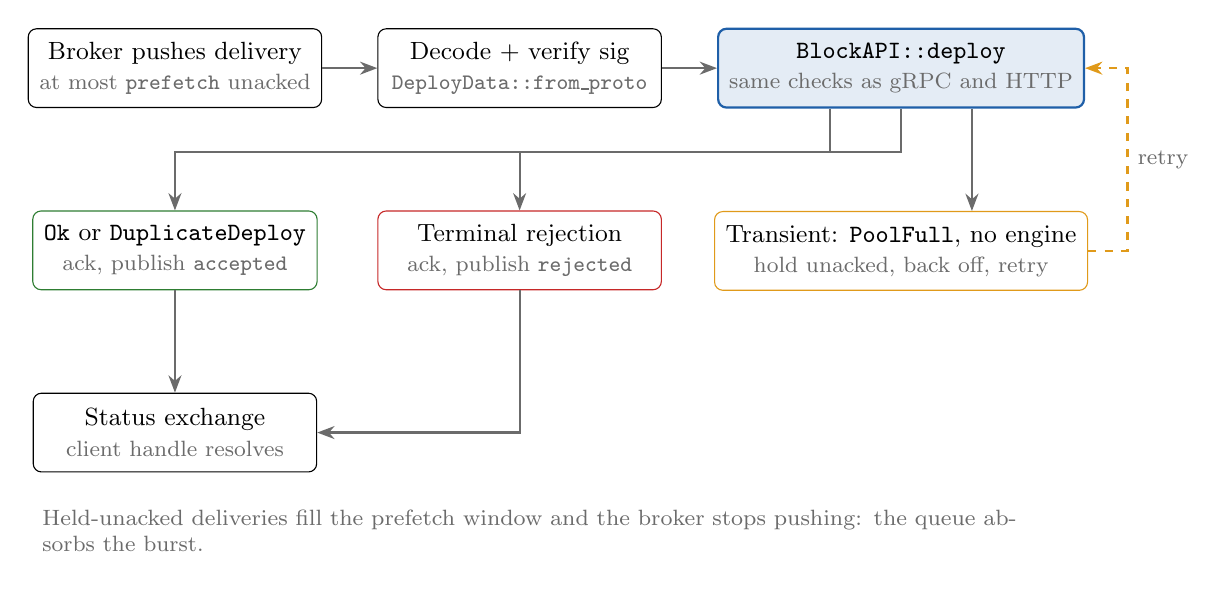
\begin{tikzpicture}[
  font=\small,
  box/.style={draw,rounded corners=3pt,align=center,minimum height=1.0cm,minimum width=3.6cm,inner sep=4pt},
  arrow/.style={-{Stealth[length=2.2mm]},quiet,thick},
  sub/.style={font=\footnotesize,color=quiet},
  node distance=0.9cm and 0.7cm,
]
\node[box] (deliv) {Broker pushes delivery\\{\subtxt at most \code{prefetch} unacked}};
\node[box,right=of deliv] (decode) {Decode + verify sig\\{\subtxt \code{DeployData::from\_proto}}};
\node[box,right=of decode,fill=accent!12,draw=accent,thick] (admit) {\textbf{\code{BlockAPI::deploy}}\\{\subtxt same checks as gRPC and HTTP}};
\node[box,below=1.3cm of deliv,draw=good] (ok) {\code{Ok} or \code{DuplicateDeploy}\\{\subtxt ack, publish \code{accepted}}};
\node[box,below=1.3cm of decode,draw=bad] (term) {Terminal rejection\\{\subtxt ack, publish \code{rejected}}};
\node[box,below=1.3cm of admit,draw=warn] (trans) {Transient: \code{PoolFull}, no engine\\{\subtxt hold unacked, back off, retry}};
\node[box,below=1.3cm of ok] (status) {Status exchange\\{\subtxt client handle resolves}};
\draw[arrow] (deliv) -- (decode);
\draw[arrow] (decode) -- (admit);
\draw[arrow] (admit.south) ++(-0.9,0) |- ($(admit.south)+(0,-0.55)$) -| (ok.north);
\draw[arrow] (admit.south) |- ($(admit.south)+(0,-0.55)$) -| (term.north);
\draw[arrow] (admit.south) ++(0.9,0) -- ($(trans.north)+(0.9,0)$);
\draw[arrow] (ok) -- (status);
\draw[arrow] (term.south) |- (status.east);
\draw[arrow,warn,dashed] (trans.east) -- ++(0.5,0) |- (admit.east) node[pos=0.25,right,font=\footnotesize,color=quiet] {retry};
\node[font=\footnotesize,color=quiet,below=0.35cm of status.south west,anchor=north west,align=left,text width=12.5cm]
  {Held-unacked deliveries fill the prefetch window and the broker stops pushing: the queue absorbs the burst.};
\end{tikzpicture}
\caption{A delivery is acked only after the node has given a verdict.}
\label{fig:flow}
\end{figure}

\paragraph{Ordering.} The queue is FIFO per publisher and the consumer processes up
to \code{prefetch} deliveries concurrently, so arrival order into the pool is
approximate. That is fine: on \dev{} the proposer orders by
$(\mathit{validAfter}, \mathit{timestamp}, \mathit{sig})$ and on v6 by
$(\mathit{timestamp}, \mathit{sig})$, neither by arrival, and there are no
per-deployer nonces. A client that needs two deploys in a fixed order waits for the
first to be \code{accepted} (or further) before publishing the second, as it must
today.

\paragraph{Back-pressure, end to end.} Three bounds, outermost first:
\code{x-max-length} with \code{reject-publish} (the client's publisher confirm comes
back as a nack and the client surfaces \code{QueueFull}); the consumer's
\code{prefetch} (how far ahead of the node the broker may push); and on the branch
\code{PoolFull} from \code{pool\_admission} (how full the node lets its pool get). On
\dev{} the third bound does not exist, so the consumer adds a soft one: it counts
\code{list\_pending\_deploys()} (\dev{} has no \code{pending\_count}; the branch's
\path{KeyValueDeployStorage::pending_count} arrives with DQ-2) against
\path{deploy-queue.max-pool-backlog} at most once a second, and treats overflow as
transient. Porting P0-09's \code{pool\_admission} to \dev{} would make the two
branches identical here and is recommended.

\begin{table}[htbp]\centering\small
\begin{tabularx}{\textwidth}{L{3.3cm} X X}
\toprule
Failure & Effect & Handling \\
\midrule
Broker down or unreachable & This node stops taking queued deploys; gRPC/HTTP ingress unaffected; other nodes unaffected (no shared broker) & lapin auto-recovery with backoff; \path{deploy_queue_connected} gauge = 0; the task is supportive, not critical: it does not take the node down (\S\ref{sec:open}) \\
Node down, broker up & Queue keeps accepting publishes up to \path{x-max-length}; deliveries wait & On restart the consumer resumes; deploys whose window closed meanwhile are terminal-rejected at ingress and reported \\
Both down (same host) & Clients get connection errors & Client policy (\S\ref{sec:client}) \\
Poison message (undecodable) & Would loop if nacked with requeue & Classified terminal: acked, \path{rejected} event, counted in \path{deploy_queue_rejected_total} with \code{reason="decode"} \\
Queue-side TTL hit & Dead-lettered to \path{f1r3node.deploy.expired} & \code{expired\{sig, stage="queue"\}} published by the DLQ watcher; the deploy would have failed the block window anyway \\
Replay by a hostile publisher & Signature valid, bytes identical & \path{DuplicateDeploy} or block-window expiry; nothing to gain \\
\bottomrule
\end{tabularx}
\caption{Failure modes and their handling.}
\label{tab:fail}
\end{table}

\section{Deploy TTL as a shard-wide parameter}
\label{sec:ttl}

The TTL is already shard-wide on both branches, so no new consensus parameter is
needed. \code{deploy-lifespan} (default 50 blocks; \path{casper/src/rust/casper_conf.rs},
\code{defaults.conf}) only seeds genesis: it is written into the PoS contract
(\code{\$\$deployLifespan\$\$} in \code{PoS.rhox} and \code{PoSV6.rhox}, via
\path{genesis/contracts/standard_deploys.rs}), served by
\path{PoS("getConsensusParameters")}, and at start-up \code{hash\_set\_casper}
(\path{casper/src/rust/casper.rs}) reads it from the approved block's post-state
through \path{token_metadata_check::read_on_chain_consensus_parameters} and
overwrites the local value unconditionally. A node whose chain state lacks it fails to
start. Every node in a shard therefore enforces the same window, and an operator sets
it once, at shard launch, through \code{casper.deploy-lifespan} on the genesis node.
The glossary (\code{docs/casper/GLOSSARY.md\#deploy-lifespan}) deliberately avoids the
word TTL because the window is counted in blocks, not time; this note uses ``block
window'' for the consensus rule and ``TTL'' only for the queue-side wall-clock bound.

\paragraph{What the window means for a buffered deploy.} The client stamps
$\mathit{validAfterBlockNumber} = h$ when it publishes. The deploy is proposable while
$h < \mathit{next}$ and $h > \mathit{next} - \mathit{lifespan}$, and ingress refuses
it once $\mathit{latest} + 1 - \mathit{lifespan} \ge h$. Time spent in the queue, time
spent in the pool, and (on v6) time withheld by the lag gate all count against the
same window. So a burst the shard cannot drain within $\mathit{lifespan}$ blocks sheds
its oldest deploys by design, each with a \code{rejected} or \code{expired} event
rather than silently. That is the intended protection against overwhelming the shard:
the buffer makes bursts survivable, the window keeps them bounded.

\paragraph{Where the window is enforced} (same on both branches unless noted):
ingress (\code{BlockAPI::deploy}); the proposer (\code{prepare\_user\_deploys} on
\dev, \code{select\_envelopes} on v6, both deleting or skipping expired deploys);
block validation (\path{Validate::transaction_expiration},
\code{future\_transaction}, \code{time\_based\_expiration}); the merger
(\path{dag_merger::split_window_closed_chains}); and on v6 the gate's
prior-status window (\path{v6/core.rs::prior}). The queue adds no enforcement point;
it only needs to stop holding messages that can no longer pass.

\paragraph{Queue-side TTL, derived not configured.} RabbitMQ can expire messages by
wall-clock age (\code{x-message-ttl}). The node derives it at start-up as
\[
  \mathrm{ttl}_{\mathrm{ms}} \;=\; \mathit{deploy\_lifespan}
  \times \mathit{heartbeat.check\_interval}_{\mathrm{ms}}
  \times \mathit{deploy\_queue.ttl\_factor},
\]
with \code{ttl-factor} defaulting to $1.0$ and $0$ meaning ``no queue-side TTL''.
\code{heartbeat.check-interval} (default 5\,s) is the shard's block cadence under
load; it already sizes \code{deploy-play-budget} the same way. The TTL is a
housekeeping bound so a dead node's queue does not fill with deploys that are
certainly expired; correctness never depends on it, because ingress re-checks the
window on every delivery. Expired messages dead-letter to
\code{f1r3node.deploy.expired}, where the DLQ watcher reports them.

\paragraph{Exposing the window to clients.} The consumer publishes a \code{shard.tip}
event on the status exchange on every new block it learns of:
\code{\{shard, block\_number, deploy\_lifespan, min\_phlo\_price,
max\_user\_deploys\_per\_block, node\}}. A subscribed client needs no HTTP call to
choose \code{validAfterBlockNumber} or to know how long its deploy can live. The same
values are available from the node's existing HTTP endpoints, so a client without a
status subscription still works.

\paragraph{Changing the window later.} Because the value lives in the PoS contract,
changing it on a running shard is a governance action (an updatable hook or a new
genesis), not a config edit, on both branches---consistent with the principle that
shard-wide parameters are set at launch and changed through multisig-authorised hooks.

\section{Component 2: the \code{f1r3node-async-rust} client}
\label{sec:client}

A Rust library crate (\code{f1r3node-async-rust}, with a thin \code{f1r3deploy}
binary over it) that signs a deploy, publishes it to one node's queue, and returns a
handle whose futures resolve as the deploy's status events arrive. It is fully async
(tokio), never blocks on the node, and never talks to the node's gRPC or HTTP ingress
for the deploy itself. It depends on the \code{models} and \code{crypto} crates for
\code{DeployData}, \code{Signed} and the signature algorithms, so signing is
byte-identical to \code{node deploy} and to \code{deploy\_runtime.rs} today.

\paragraph{Public API (sketch).}
\begin{lstlisting}
let signer = Secp256k1Signer::from_hex(&private_key_hex)?;
let client = NodeClient::connect(NodeEndpoint {
    amqp: "amqps://deployer@validator-1.example:5671/%2f".parse()?,
    shard_id: "asi-testnet".into(),
    queue: QueueName::default_for("asi-testnet", &validator_pk),
    status: StatusSubscription::Deployer,    // <pk>.# on the status exchange
}).await?;

let handle: DeployHandle = client
    .deploy(DeployRequest {
        term,
        phlo_limit: 100_000,
        phlo_price: PhloPrice::AtLeastFloor,  // or Exact(n)
        valid_after: ValidAfter::LatestTip,   // from the last shard.tip; or Explicit(h)
        expiration_timestamp: None,
        cosigners: vec![],                    // v6: required cosigners
    }, &signer)
    .await?;                                  // resolves on the broker's publish confirm

handle.id();                                  // DeployId = sig bytes, hex
handle.accepted().await?;                     // Accepted | Rejected(reason) | Deferred(reason)
let mut events = handle.events();             // Stream<DeployEvent>
handle.finalized().await?;                    // Ok(receipt) | Err(Expired | Rejected | Discarded)
\end{lstlisting}

\paragraph{Publish semantics.} \code{deploy()} opens a confirm-mode channel and
publishes with \code{mandatory = true} and \code{delivery\_mode = persistent}. It
resolves \code{Ok(handle)} on a broker ack, \code{Err(QueueFull)} on a nack caused
by \code{x-max-length} with \code{reject-publish}, \code{Err(Unroutable)} if the
node has not declared its queue yet (the exchange returns the message), and
\code{Err(Broker(\_))} on connection failure. None of these errors means the deploy
was seen by the node, so all are safe to retry with the same bytes. After a broker
ack the deploy is durably queued; a client crash from then on loses nothing, and the
handle can be reconstructed from the signature (\code{client.attach(deploy\_id)}).

\paragraph{Status tracking.} The handle is driven by the status exchange. On connect
the client declares an exclusive, auto-delete queue bound to
\code{f1r3node.deploy.status} with routing key \code{<deployer-pk-hex>.\#} (one
subscription covers all of a deployer's deploys) and to \code{shard.tip}.
\begin{center}\small
\begin{tabularx}{\textwidth}{X L{3.1cm} L{1.8cm} L{1.3cm} L{1.4cm}}
\toprule
Event & Source & Terminal? & \dev & v6 \\
\midrule
\path{accepted} & consumer, after \path{BlockAPI::deploy} & no & yes & yes \\
\code{rejected\{reason, terminal\}} & consumer & yes & yes & yes \\
\code{deferred\{reason\}} & consumer & no & yes & yes \\
\code{included\{block\}} & consumer, from the node's \code{BlockAdded} event & no & yes & yes \\
\code{gate\_rejected\{reason\}} (offer removed from pool; same bytes may be resubmitted) & node lifecycle hook & yes, retryable & n/a & phase 2 \\
\code{finalized\{block, cost, errored\}} & consumer, from the node's \code{BlockFinalised} event & yes & yes & yes \\
\path{expired} / \path{discarded} / receipts & node lifecycle hook (\path{finality/deploy_lifecycle.rs} verdicts, v6 offer status) & yes & phase 2 & phase 2 \\
\path{shard.tip} & consumer, per new block & n/a & yes & yes \\
\bottomrule
\end{tabularx}
\end{center}
Phase 1 ships \code{accepted}, \code{rejected}, \code{deferred}, \code{shard.tip},
\code{included} and \code{finalized}: the last two come from the node's existing
event bus (\code{F1r3flyEvents}: \code{BlockAdded}, \code{BlockFinalised}), so the
consumer emits them without touching Casper internals. Expiry is detected client-side
from \code{shard.tip} passing \code{validAfter + deploy\_lifespan} with no inclusion
seen; an endpoint with an HTTP base URL also polls
\path{/api/deploy-finalization-status/{sig}} as a fallback. Phase~2 adds the v6
offer-status events. The handle's API does not change between phases.

\paragraph{Retry policy, built in and conservative.} The client retries only
publish-side failures with the same bytes. After a terminal \code{rejected},
\code{discarded} or \code{expired} it never republishes the same signature: on v6 an
\code{AlreadyIncluded}/\code{Discarded} signature is dead for its window (FX-17), and
on both branches a block-window rejection means a new \code{validAfterBlockNumber},
hence a new signature. \code{handle.resign\_and\_retry(\&signer)} is the explicit,
opt-in path that builds a fresh deploy (new timestamp and \code{validAfter}) and
publishes it. \code{gate\_rejected} on v6 is the one retryable-with-same-bytes
terminal state; the client exposes \code{handle.resubmit()} for it.

\paragraph{Choosing a node.} The queue is node-local and the default client talks to
exactly one node. \code{ShardClient} is a thin optional layer over several
\code{NodeClient}s with one policy: sticky to a preferred node, failing over to the
next on \code{Broker}/\code{Unroutable} errors---never on \code{QueueFull}, which is
the shard telling the client to slow down. It does not spread one client's deploys
across nodes; a deploy's status subscription lives on the node that took it.

\paragraph{Cosigned deploys (v6).} \code{client.prepare(request, \&signer)} returns
the envelope awaiting cosigners; \code{cosign(envelope, \&cosigner)} adds a
\code{DeployCosignature} using the FX-3 preimage; \code{deploy\_envelope(envelope)}
publishes. The CLI mirrors the branch's \code{node cosign prepare | sign | submit}.

\paragraph{Binary.} \code{f1r3deploy --node amqps://\ldots\ --shard asi-testnet
--key-file k.pem --phlo-limit 100000 file.rho [--wait accepted|finalized]} prints
the deploy id and, with \code{--wait}, the terminal event as JSON. A
\code{f1r3deploy burst --clients N --rate R --duration D} subcommand drives the soak
test in \S\ref{sec:plan}.

\paragraph{Where it lives.} A new repository \code{F1R3FLY-io/f1r3node-async-rust},
Apache~2.0 like the node, depending on \code{f1r3node-rust} crates by git revision.
Alternative: a \path{client/} workspace crate inside \code{f1r3node-rust}, which
keeps versions in lock-step but ties client releases to node releases
(\S\ref{sec:open}).

\section{Branch compatibility}

One implementation serves both branches because everything branch-specific sits
behind \code{BlockAPI::deploy} and the \code{DeployDataProto} decoder, and the
consumer touches neither.
\begin{center}\small
\begin{tabularx}{\textwidth}{L{3.4cm} X X}
\toprule
Concern & Shared & Per branch \\
\midrule
Consumer task, topology, ack policy, status publisher, config section & yes & --- \\
Decoding the body & \path{prost} decode of \path{DeployDataProto} from the branch's own \path{models} crate & \dev{} ignores unknown fields 15--16; the branch reads them \\
Signature and cosignature verification & \path{DeployData::from_proto} & the branch's \path{from_proto} also runs \path{with_complete_cosignatures} \\
The admission call & \code{BlockAPI::deploy(engine\_cell, signed, trigger\_propose\_f, read\_only, shard\_name)} & argument list identical on both; the branch's \path{trigger_propose_f} is the coalescing one \\
Outcome classification & one \code{classify(\&err) -> Class} function & \path{PoolFull} exists only on the branch; on \dev{} the arm is unreachable and the soft pool bound stands in \\
Status events & same schema & \path{gate_rejected}, \path{discarded}, receipts only on v6 (phase 2) \\
\bottomrule
\end{tabularx}
\end{center}
Mechanically: the patch is written once against \dev{} and cherry-picked onto \ote{}
(or its successor integration branch). The branch's \code{block\_api.rs} has moved
lines but the same signature, so the conflict surface is \code{setup.rs} wiring and
\code{defaults.conf}. The client crate builds against either branch's
\code{models}/\code{crypto} at a pinned revision; because the branch's proto is a
strict superset, a client built against the branch can publish to a \dev{} shard
(fields 15--16 empty) and a client built against \dev{} can publish uncosigned deploys
to a v6 shard. The design deliberately does \emph{not} reach into v6 internals (gate,
policy, seals): a buffered v6 deploy still meets the gate at proposal, exactly as an
unbuffered one does, so nothing here needs to change when the cost-accounting branch
lands in \dev.

\section{Operations}

\paragraph{Configuration} --- a new node-local section in \code{defaults.conf} /
\code{NodeConf} (not a consensus parameter; per-node values may differ, like
\code{deploy-play-budget}):
\begin{lstlisting}
deploy-queue {
  enabled = false                 # off by default; gRPC/HTTP ingress unchanged
  amqp-url = "amqp://127.0.0.1:5672/%2f"
  queue-name = ""                 # "" = f1r3node.deploy.<shard>.<pk-prefix>
  prefetch = 64                   # unacked deliveries the broker may push
  max-length = 100000             # x-max-length; overflow = reject-publish
  ttl-factor = 1.0                # x-message-ttl = lifespan * check-interval * factor; 0 = none
  max-pool-backlog = 8192         # dev only: soft bound (branch uses pool_admission)
  max-backoff = 30 seconds        # retry ceiling for transient outcomes
  status-exchange = "f1r3node.deploy.status"
  tls { enabled = false, ca-file = "", cert-file = "", key-file = "" }
}
\end{lstlisting}
CLI overrides follow the \code{config\_mapper.rs} pattern for each key.
\code{enabled = true} with an unreachable broker logs an error and retries; it does
not stop the node.

\paragraph{Running the broker.} One RabbitMQ container per node:
\path{docker/shard.yml} gains a \code{rabbitmq-<n>} service per validator, with the
management plugin bound to localhost only; \path{docker/standalone.yml} gains one.
The \code{ign1t10n} installer (local macOS shard) adds a RabbitMQ install step and the
three config lines. Production guidance: broker and node on the same host or pod so
``node-local'' holds physically; a broker shared between validators is a
configuration error the node detects at start-up (queue name already bound to another
validator's consumer tag) and refuses.

\paragraph{Security.} The deploy is signed end to end, so a compromised broker can
delay, drop or replay but not forge; replay is idempotent. AMQP credentials: one
publishing user per shard (or per client organisation) with \code{write} on
\code{f1r3node.deploy} and \code{read} on \code{f1r3node.deploy.status} only; the
node's user alone has \code{configure}. TLS (\code{amqps}) on any non-loopback
listener, reusing the node's TLS material. Status events carry no term text, only
signatures, reasons and block references.

\paragraph{Metrics} (Prometheus, beside the node's existing ones):
\path{deploy_queue_connected}, \path{deploy_queue_depth},
\code{deploy\_queue\_consumed\_total\{outcome\}},
\code{deploy\_queue\_rejected\_total\{reason\}},
\path{deploy_queue_deferred_seconds} (time a delivery waited unacked),
\path{deploy_queue_admission_seconds} (\path{BlockAPI::deploy} latency),
\path{deploy_queue_stalled}, \path{deploy_queue_dead_lettered_total}. A new
\code{GET /api/deploy-queue} returns \code{\{enabled, connected, depth, prefetch,
max\_length, ttl\_ms, consumed\_total\}} so a client or operator can see the buffer
without broker credentials.

\clearpage
\section{Development plan}
\label{sec:plan}

Five patches, each independently testable, in the lane style of the rev-stacks plan
(\path{patch/<ID>} branches, \code{[agent]} commits, decisions logged under
\path{docs/designs/deploy-queue/decisions/}). DQ-1 and DQ-3 can run in parallel once
the message contract in \S\ref{sec:node} is frozen.
{\small
\begin{xltabular}{\textwidth}{L{1.9cm} X L{2.8cm} X}
\toprule
Patch & Scope & Branch(es) & Acceptance \\
\midrule
\endhead
DQ-1 node consumer & \path{deploy-queue} config + CLI mapping; \path{DeployQueueConsumer} (lapin), topology declaration, classify + ack policy, \path{shard.tip}/\path{accepted}/\path{rejected}/\path{deferred} publisher, metrics, \code{GET /api/deploy-queue} & \dev, then cherry-pick to \path{feature/rev-stacks-ote} & With \code{enabled = false} behaviour is unchanged. With a broker up, a deploy published as raw proto is admitted and appears in \path{/api/pending-deploys}; redelivery after a kill between admission and ack yields \path{duplicate}, not a second pool entry; each terminal class produces ack + \path{rejected}; \path{PoolFull} (branch) and the soft bound (\dev) hold the delivery unacked and the broker stops at \path{prefetch} \\
DQ-2 pool cap on \dev{} (optional, recommended) & Port P0-09/P0-10 \path{pool_admission}, \path{PoolFull}, HTTP 503 \path{deploy_pool_full} & \dev & The branch's P0-09 tests pass on \dev; the soft bound becomes dead code and is removed \\
DQ-3 client crate & \path{f1r3node-async-rust}: \path{NodeClient}, \path{DeployRequest}, \path{DeployHandle}, status subscription, confirm-mode publishing, error taxonomy, \path{ShardClient} failover, \path{f1r3deploy} incl.\ \path{burst} & new repo, pinned to each branch & Signs byte-identically to \code{node deploy} (golden test against \path{deploy_runtime.rs}); \path{QueueFull}, \path{Unroutable}, \path{Broker} surfaced and retried correctly; \path{accepted()} resolves from the event stream; polling fallback resolves \path{finalized()} on both branches \\
DQ-4 packaging & \path{docker/shard.yml}, \path{docker/standalone.yml} broker services; \path{ign1t10n} step; operator page in \path{docs/node/}; glossary anchors \code{\#deploy-queue}, \code{\#status-exchange} & \dev & \code{docker compose -f docker/shard.yml up} brings up three validators each with its own broker; \path{f1r3deploy} against any one of them succeeds \\
DQ-5 lifecycle events (phase 2) & Hook in \path{finality/deploy_lifecycle.rs} (both) and the v6 offer-status path to publish \path{proposed}, \path{gate_rejected}, \path{finalized}, \path{expired}, \path{discarded} & both & The handle resolves \path{finalized()} without polling; events match \path{/api/deploy-finalization-status} and \code{/deploy/offered/\{id\}/receipt} in a randomized comparison \\
\bottomrule
\end{xltabular}
}

\paragraph{Tests.}
\begin{itemize}[leftmargin=2em]
  \item Unit: the classification table (every \code{DeployError}/\code{CasperError}
    arm has a class); TTL derivation; queue-name derivation; proto round-trip with
    fields 15--16 present on \dev's decoder (must survive as raw bytes, never be
    re-encoded).
  \item Integration: RabbitMQ in \code{testcontainers}; the three-validator
    \path{docker/shard.yml}; crash between admit and ack; broker restart mid-burst
    (auto-recovery); node restart with a full queue.
  \item Soak, the point of the exercise: \code{f1r3deploy burst} from $N$ clients
    against one node and against all three, at rates above and below what the shard
    drains, measuring admission latency, pool depth, time-to-finalized, and the
    fraction shed by the block window. Run on both branches through
    \path{scripts/casper-soak}; the v6 run is the one that matters for the ASI
    TestNet and should follow the Track~B handoff candidate, not precede it. Pass
    criteria: no validator stall across the run; no deploy lost without a terminal
    event; shed fraction $0$ at a sustainable rate and bounded by $\mathit{lifespan}$
    at overload.
\end{itemize}

\paragraph{Order.} DQ-1 on \dev{} first (the merge target), DQ-3 against it, DQ-4 to
make the three-node test reproducible, then the cherry-pick of DQ-1 onto the
cost-accounting branch and the v6 soak; DQ-2 and DQ-5 follow. Nothing merges to \dev{}
until the soak passes on both.

\paragraph{Implementation status (7 November 2026).} DQ-1, DQ-3 and DQ-4 are
implemented on a branch from \dev{} \code{a79a6ce}: \path{node/src/rust/deploy_queue/}
(config, naming, classify, consumer, status, lifecycle), the \code{deploy-queue}
section of \code{defaults.conf}, \path{GET /api/deploy-queue}, the docker overlays
\path{docker/deploy-queue.yml} and \path{docker/deploy-queue-standalone.yml}, and the
operator page \path{docs/node/deploy-queue.md}; the client lives in
\code{f1r3node-async-rust} with the \code{f1r3deploy} binary. Verified against a live
RabbitMQ 3.12: the client's publish confirms, \code{QueueFull}, \code{Unroutable} and
the accepted/rejected round trip; the node consumer's topology declaration, hold-unacked
behaviour on a transient verdict with a \code{deferred} event, and terminal handling of
undecodable bytes. Not yet run: the three-validator soak (DQ-1 end to end against a
running shard) and the cherry-pick onto \ote. One design correction surfaced by the
broker: the per-deploy routing key is \path{<deployer>.<sig-prefix>}, not the full
signature.

\section{Open questions and decisions needed}
\label{sec:open}

Each has a recommended default so work can start; answers that differ change the
patch, not the design.
\begin{enumerate}[leftmargin=2em]
  \item \textbf{Broker outage and the node.} Recommended: the consumer is a
    supportive task; a broker failure degrades this node to gRPC/HTTP ingress and
    alarms, never stops the node. Alternative: treat it as critical so a
    buffered-only deployment fails loudly.
  \item \textbf{Queue-only mode.} Should a shard be able to close gRPC/HTTP
    \code{doDeploy} so every deploy is buffered? Recommended: a
    \code{deploy-queue.exclusive = false} flag; when on, the direct endpoints return
    503 \code{use\_deploy\_queue} with the queue name.
  \item \textbf{Port the pool cap to \dev{} (DQ-2).} Recommended yes: both branches
    then share the same back-pressure signal and the soft bound goes away.
  \item \textbf{Status events in phase 1.} Recommended: ingress verdicts +
    \code{shard.tip} only; lifecycle events in DQ-5 after the Track~B handoff, so the
    consumer does not touch the finalizer while that lane is landing.
  \item \textbf{Client repository.} Recommended: a separate
    \path{F1R3FLY-io/f1r3node-async-rust} repo pinned to node revisions, since
    clients release on their own cadence and ASI's TestNet users will consume it
    independently of node builds. Alternative: a \path{client/} workspace crate.
  \item \textbf{Early elaboration check on v6.} Running
    \code{source\_to\_adt\_elaborated} in the consumer would reject malformed seal
    forms immediately instead of letting them become \code{Discarded} network-wide,
    at the cost of CPU per delivery and a dependency on the rholang crate's
    elaborator. Recommended: off by default, behind \code{deploy-queue.elaborate},
    revisited after the v6 soak shows how often it would fire.
  \item \textbf{Queue-side TTL.} Recommended: derived (\code{ttl-factor = 1.0})
    rather than unset, so a dead node's queue cannot fill with certainly-expired
    deploys; \code{0} if operators prefer the ingress check to be the only expiry.
  \item \textbf{Per-deployer fairness.} A single client can fill a node's queue and
    starve others until \code{x-max-length} pushes back on everyone; RabbitMQ has no
    per-publisher quota. Options: accept it (node-local queue, node operator chooses
    its clients); or per-deployer queues bound to the same exchange with the
    consumer round-robining across them. Recommended: accept it for phase 1, record
    the per-deployer variant as the follow-up if the soak shows starvation.
  \item \textbf{Naming and home.} \code{f1r3node-async-rust} is the working name;
    \code{f1r3node-client} is the alternative. Also whether this note is checked into
    \path{docs/designs/deploy-queue/} on \dev{} as the lane's design record.
\end{enumerate}

\section*{Sources}
\begin{itemize}[leftmargin=2em]\small
  \item \path{F1R3FLY-io/f1r3node-rust}, \dev{} at \code{a79a6ce} and \ote{} at
    \code{4c9853b}: \path{casper/src/rust/api/block_api.rs},
    \path{engine/multi_parent_casper/block_admission.rs},
    \path{blocks/proposer/block_creator.rs}, \path{util/deploy_window.rs},
    \code{casper.rs} (\path{hash_set_casper}), \code{v6/\{propose,gate,core,
    resource\_policy,genesis\_policy\}.rs}, \code{node/src/rust/runtime/\{setup,
    node\_runtime\}.rs}, \path{node/src/main/resources/defaults.conf},
    \path{casper/src/main/resources/PoS.rhox}.
  \item \path{docs/casper/GLOSSARY.md} (\code{\#deploy-admission},
    \code{\#deploy-lifespan}, \code{\#rejected-deploy-buffer},
    \code{\#deploy-lifecycle}); \path{docs/node/api-reference.md};
    \path{docs/rholang/18-deployment-workflow.md}; \path{docs/data-flows/README.md}.
  \item \path{docs/rev-stacks/decisions/}: FX-3, FX-8b, FX-17, FX-21, FX-22, P0-01,
    P0-09, P0-10, P1-13, P2-07, P2-10; \path{docs/plans/v6-order-then-execute-tranche-1.md}.
  \item ``F1R3FLY.io Deployment Architecture'' (PDF, Google Drive, 2026-11-07).
  \item \code{lapin} 4.10 documentation, \url{https://docs.rs/lapin}.
\end{itemize}

\end{document}
